\section{Attacchi alle funzioni hash}

%------------------------------------------------
\begin{frame}
	\frametitle{Paradosso del compleanno}

	Il paradosso afferma che la probabilità che almeno due persone in un gruppo compi il proprio compleanno lo stesso giorno è \textbf{largamente superiore} a quanto potrebbe dire l'intuito

	Supponiamo che ci siano 365 giorni in un anno e che ogni compleanno sia \textbf{equiprobabile}, con p numero di persone nel gruppo.

	\[
		P(\text{nessuna collisione}) = \frac{365}{365} \times \frac{364}{365} \times \frac{363}{365} \times \cdots \times \frac{365 - p + 1}{365}
	\]

	\[
		P(\text{nessuna collisione}) = \frac{365!}{365^(p-1) (365 - n)!}
	\]

\end{frame}

\begin{frame}
	\frametitle{Paradosso del compleanno P2}

	La probabilità di \textit{almeno una} collisione è:

	\[
		P(\text{almeno una collisione}) = 1 - P(\text{nessuna collisione})
	\]

	\[
		P(\text{almeno una collisione}) = 1 - \frac{365!}{365^(p-1) (365 - n)!}
	\]

\end{frame}


\begin{frame}
	\frametitle{Paradosso del compleanno P3}

	Per avere il 50\% di probabilità di trovare almeno una collisione, \textbf{bastano 23 persone}.

	\begin{center}
		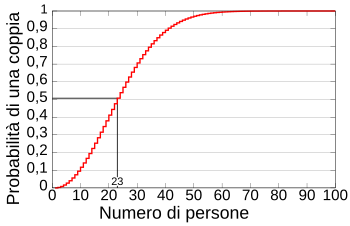
\includegraphics[width=0.8\textwidth]{img/2-img/Birthday_Paradox_IT.png}
	\end{center}

\end{frame}

\begin{frame}
	\frametitle{Paradosso del compleanno nelle funzioni hash}

	Dato una funzione hash \(H\) che mappa il proprio output su N bit sarà reputata insicura quando \textbf{si potrà facilmente generare $2^{N/2}$ risultati}.

	\vspace{1cm}

	Nel caso di SHA-1, dato che l'output è a 160 bit, se si potesse generare $2^{80}$ con un'\textbf{attacco a forza bruta} si avrebbe una probabilità di trvare una collissione \textbf{\> 50\%}.
\end{frame}


\begin{frame}
	\frametitle{Primi attacchi a SHA-1}
	Nel \textbf{2005} il team di ricerca della Shandong University annunciò il \textbf{primo attacco a SHA-1}, con una complessità di \(2^{69}\) operazioni.
	Pochi mesi dopo fu annunciato un attacco a \(2^{63}\) operazioni.
	Un normale attacco che sfrutta il paradosso del compleanno avrebbe una complessità di \(2^{80}\) operazioni come visto prima.

	\vspace{1cm}

	Nel 1999 DESCracker era già capace di eseguire \(2^{56}\) operazioni in 56 ore, seguendo la legge di Moore i tempi di calcolo dovevano già essere alla portata di governi e organizzazioni criminali nel 2010.
\end{frame}


\begin{frame}
	\frametitle{Google SHAttered}

	In 2 anni hanno trovato un modo per generare \textbf{due PDF diversi con lo stesso hash SHA-1}.
	Fino a quel momento \textbf{l'industria era ancora poco propensa ad abbandonare SHA-1} per la mancanza di un \textbf{esempio pratico} che dimostrasse la collisione.
	\begin{itemize}
		\item 9 quantiglioni (\(9,223,372,036,854,775,808\)) di calcoli SHA-1 in totale
		\item \textbf{6.500 anni di calcolo CPU} per completare la prima fase dell'attacco
		\item \textbf{110 anni di calcolo GPU} per completare la seconda fase
	\end{itemize}

	L'attacco SHA-1 shattered è ancora più di \textbf{100.000 volte più veloce di un attacco brute force}, che rimane impraticabile (\(2^{63}\) operazioni).
\end{frame}

\begin{frame}
	\frametitle{Google SHAttered: Come è stato ottenuto}

	L'obiettivo è stato quello di trovare coppie di blocchi di dati che, quando \textbf{concatenati con un prefisso P e qualsiasi suffisso S}, producono hash identico.

	Si procede trovando la prima coppia di blocchi di dati \(M_{1}^{(1)}, M_{1}^{(2)}\) che portano ad una \textbf{quasi collisione}.

	\[
		\text{SHA-1} \left( P \parallel M_{1}^{(1)} \parallel M_{2}^{(1)} \parallel S \right) = \text{SHA-1} \left( P \parallel M_{1}^{(2)} \parallel M_{2}^{(2)} \parallel S \right).
	\]


	Successivamente si sfrutta il primo per trovare un secondo blocco \(M_{2}^{(1)}, M_{2}^{(2)}\) in cui si possa trovare una vera collisione.
	La difficoltà di trovare il secondo blocco è significativamente più alta, e spesso richiede più risorse computazionali e strategie sofisticate rispetto al primo.

\end{frame}

\begin{frame}
	\frametitle{Creazione del PDF}

	Si è poi sfruttata la flessibilità del formato PDF e JPEG per creare i 2 documenti che contenessero i blocchi per generare la collissione.

	\begin{center}
		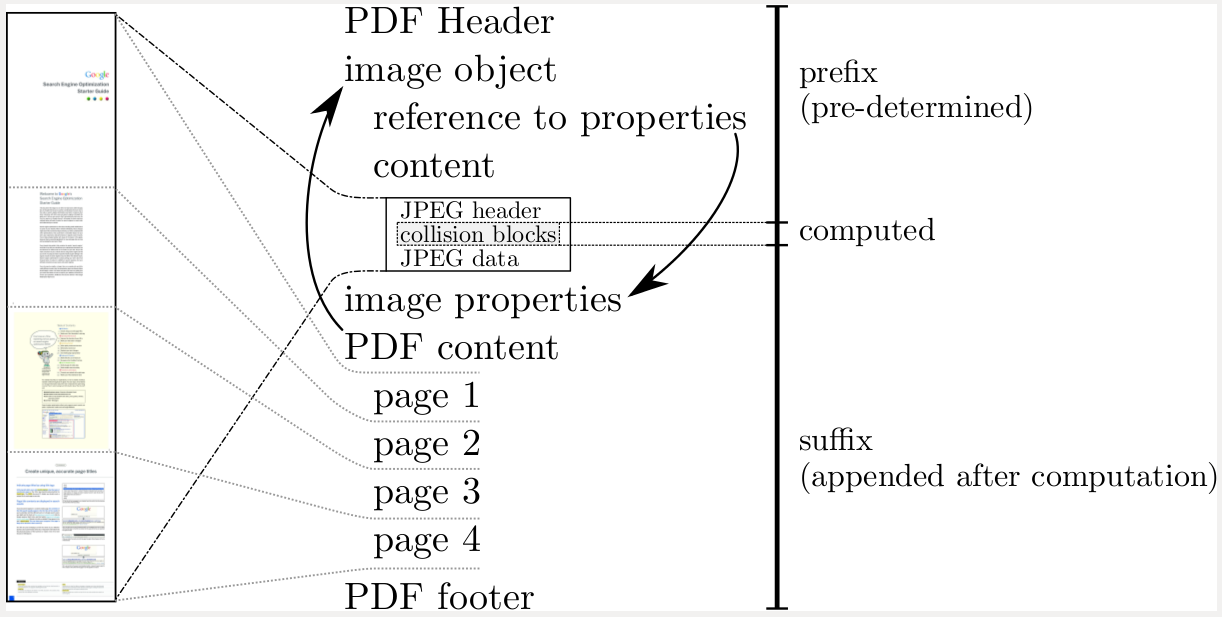
\includegraphics[width=0.8\textwidth]{img/2-img/pdf_format.png}
	\end{center}

\end{frame}